\label{sec:experiment}

\subsection{Datasets}
In short, their motivation for creation of the \texttt{AUTSL} dataset is to replicate the real–world scenarios when using sign languages.
The dataset contains frequently used vocabularies in spoken language, and keep the dataset balanced in terms of motion characteristics and time taken to complete a word.
\textbf{Table \ref{tab:AUTSL_description}} below shows an overview of the dataset.

\begin{table}[H]
\centering\small
\begin{tabular}{@{}c c@{}}
\toprule
\textbf{Property} & \textbf{Description}  \\
\midrule
Number of signs & $226$  \\
Number of signers & $43$ \\
Total samples & $38,336$ \\
Number of different backgrounds &  $20$ \\
Mean sample per sign & $169.6$ \\
Modalities & RGB, depth, skeleton \\
RGB and depth resolution & $512 \times 512$ \\
FPS & 30 \\
\bottomrule
\end{tabular}
\caption{Statistics of AUTSL dataset \cite{sincan2020autsl}.}
\label{tab:AUTSL_description}
\end{table}

Regarding challenges, the videos span a wide variety of static and dynamic backgrounds, the latter containing objects moving behind the signer.
The authors further selected signs that are very similar in motion and separated only by subtle gestures, included compound signs built from simpler ones, and recruited signers of differing backgrounds, so that personal signing style varies across the dataset.


In this experiment, we leverage the available \texttt{AUTSL} dataset given in Kaggle, accessible via \href{https://www.kaggle.com/datasets/sttaseen/autsl}{this link}.
This dataset only comprises of RGB-colored videos, for a comprehensive dataset of \texttt{AUTSL}, including different video formats of the same data, refer to \href{https://cvml.ankara.edu.tr/datasets/}{this link}.
Therefore, by utilisation of Kaggle dataset, we limit ourselves to benchmark \texttt{X3D} performance on RGB–colored videos. Lastly, the downloaded data was already partitioned, and thus, we shall not split the dataset by our own.

\begin{table}[H]
\centering\small
\begin{tabular}{@{}c c c@{}}
\toprule
\textbf{Set} & \textbf{Number of samples} & \textbf{Percentage}  \\
\midrule
Train & $28,142$ & $77.5\%$ \\
Validation & $4,418$ & $12.2\%$ \\
Test & $3,742$ & $10.3\%$ \\
\midrule
Total & $36,302$ & 100\% \\
\bottomrule
\end{tabular}
\caption{Number of samples inspected directly from the dataset.}
\label{tab:AUTSL_samples}
\end{table}

Apparently, \textbf{Table \ref{tab:AUTSL_description}} and \textbf{Table \ref{tab:AUTSL_samples}} differ in the total number of samples, suggesting a data shift between the Kaggle release and the original.
We therefore re–inspect the dataset from its filenames in \textbf{Figure \ref{fig:data-inspect-1}} and \textbf{Figure \ref{fig:data-inspect-2}}, which still count every clip.
Of these, $11$ are truncated and cannot be decoded, i.e. $10$ in train and $1$ in test, and are excluded from both training and testing, leaving the $28{,}132$ and $3{,}741$ clips actually used.

\begin{figure}[H]
    \centering
    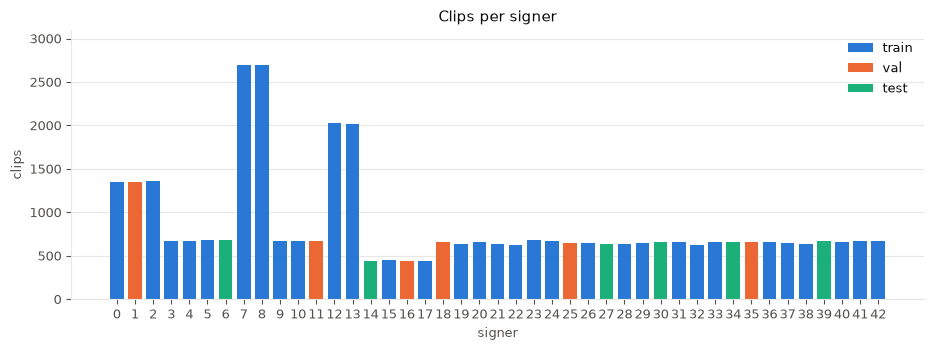
\includegraphics[width=1\textwidth]{figures/data_inspect_1.png}
    \caption{Inspection of number of clips produced by each signer.}
    \label{fig:data-inspect-1}
\end{figure}

\begin{figure}[H]
    \centering
    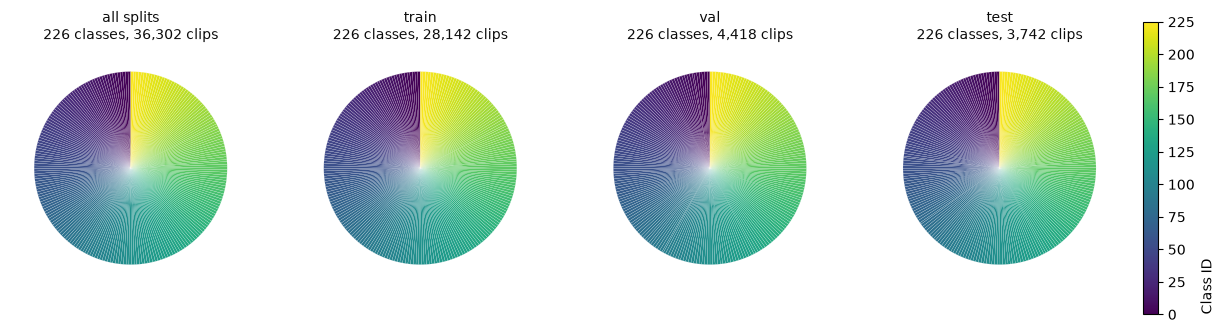
\includegraphics[width=\textwidth]{figures/data_inspect_2.png}
    \caption{Distribution of sign classes across the dataset splits. Every split covers all $226$ classes.
    \textbf{All splits:} $36{,}302$ clips, with min $121$, median $162$, mean $160.6$ and max $164$ clips per class.
    \textbf{train:} $28{,}142$ clips (min $90$, median $126$, mean $124.5$, max $127$)
    \textbf{validation:} $4{,}418$ clips (min $12$, median $20$, mean $19.5$, max $20$)
    \textbf{test:} $3{,}742$ clips (min $10$, median $17$, mean $16.6$, max $17$).}
    \label{fig:data-inspect-2}
\end{figure}

\paragraph{Dataset building.} According to the models' sizes in \href{https://github.com/facebookresearch/pytorchvideo/blob/f3142bb05cdb56af0704ab6f0adfb0c7bbafe4a0/pytorchvideo/models/x3d.py#L539}{this code}, we adopt the clip geometry summarised in \textbf{Table \ref{tab:model_sizes}}.
\begin{table}[H]
    \centering\small
    \begin{tabular}{@{}c c c@{}}
    \toprule
    \textbf{Model size} & \texttt{num\_frames} & \texttt{crop\_size}  \\
    \midrule
    \texttt{X3D\_XS} & $4$ & $160$  \\
    \texttt{X3D\_S} & $13$ & $160$  \\
    \texttt{X3D\_M} & $16$ & $224$  \\
    \bottomrule
    \end{tabular}
    \caption{Number of frames and crop size for each video.}
    \label{tab:model_sizes}
\end{table}
\texttt{AUTSL} dataset must be built with the matching \texttt{num\_frames} and \texttt{crop\_size}, otherwise the weights load but the model sees inputs it was never trained for.

\subsection{Implementation details}
\label{sec:implementation}
% Describe the experimental environment


In this experiment, we do not benchmark the model against other methods. Alternatively, we benchmark different fine-tuning approaches of different models' sizes.

In the original codebase, \texttt{X3D} was pretrained on \texttt{Kinetics--400} dataset \cite{kay2017kinetics}, and thus the final \texttt{softmax} layer does not match the number of classes in \texttt{AUTSL} dataset.
Therefore, we replace the final linear projection layer, to reduce the number of classes.
Formally, let $g(\mathbf x)$ is the final fully connected layer of pretrained \texttt{X3D}, given by:
\begin{align}
    g: \mathbb R^{k} \mapsto \mathbb R^{400}
\end{align}
We shall replace it by:
\begin{align}
    g: \mathbb R^k \mapsto \mathbb R^{226}
\end{align}

The remaining settings are as follows.
\begin{itemize}[topsep=2pt, itemsep=2pt]
    \item \textbf{Data.} The \texttt{AUTSL} train split, i.e. $28{,}142 - 10 = 28{,}132$ clips over $226$ classes, unless a subset is configured.
    \item \textbf{Preprocessing.} Uniform temporal subsampling to the variant's clip length, resizing to its crop size, random horizontal flip, scaling to $[0,1]$ and per--channel normalisation with mean $0.45$ and standard deviation $0.225$.
    \item \textbf{Initialisation.} \texttt{Kinetics--400} weights for the backbone, and a freshly initialised linear head.
    \item \textbf{Optimisation.} Cross--entropy loss with \texttt{Adam}. About fine–tuning different components, frozen blocks are excluded from the optimiser and held in evaluation mode, so that their \texttt{BatchNorm} running statistics do not drift.
    \item \textbf{Hyperparameters.} Epochs = 100, batch size = 16 and learning rate = $10^{-4}$.
    \item \textbf{Hardware.} AMD EPYC 7402P (24 cores - 48 threads), 256 GB DDR4 RAM and 4x NVIDIA A100 (40GB HBM2 each).
\end{itemize}




\subsection{Evaluation metrics}
\label{sec:metrics}

Since \texttt{X3D} is designed around an accuracy–complexity trade-off rather than accuracy alone \cite{feichtenhofer2020x3d}, we report metrics along two axes, i.e. how well a model recognises signs, and how expensive it is to store and to evaluate.
% Reporting only the former would conceal exactly the property that motivates this family of networks \cite{tan2019efficientnet, MoViNets}.

\paragraph{Top–$k$ accuracy.}
Let the test split be $\mathcal D = \{(\mathbf V_i, y_i)\}_{i=1}^{N}$, where $\mathbf V_i$ is a clip and $y_i \in \{1, \ldots, C\}$ is its sign label, $C = 226$ being the number of classes.
For each clip the network, i.e. the final \texttt{softmax} layer, produces a score vector $\mathbf z_i = (z_{i1}, \ldots, z_{iC}) \in \mathbb R^C$, and we write $\mathcal R_k(\mathbf V_i) \subseteq \{1, \ldots, C\}$ to denote the subset of $k \le C$ classes receiving the largest scores.
The top–$k$ accuracy:
\begin{align}
    \text{top--}k = \frac{1}{N} \sum_{i=1}^{N} \mathbf 1 \left\{ y_i \in \mathcal R_k(\mathbf V_i) \right\},
\end{align}
where $\mathbf 1\{\cdot\}$ denotes the indicator function.
% As the \texttt{softmax} map is strictly increasing, it preserves the ordering of $\mathbf z_i$, and hence $\mathcal R_k$ may equivalently be taken over logits.

We evaluate $k \in \{1, 3, 5\}$, and note that
$\mathcal R_1 \subseteq \mathcal R_3 \subseteq \mathcal R_5 \Rightarrow \text{Top--}1 \le \text{Top--}3 \le \text{Top--}5$.
Top–1 is the strict accuracy, i.e. the fraction of clips whose most probable class is correct, and is the quantity of practical interest for a recognition system.
Top–5 is the conventional companion metric on \texttt{Kinetics–400} \cite{kay2017kinetics} and \texttt{ImageNet} \cite{Russakovsky2015}.
Top–3 is included to give balance between strict metric top–1 and easy metric top–5.
The margin between Top–1 and Top–3 therefore diagnoses the nature of the residual errors, i.e. a small margin indicates genuine failures, whereas a large one indicates near misses within a small group of mutually confusable signs.

\paragraph{Total and trainable parameters.}
Let $\theta$ be the full set of parameters of a model and $\theta_{\text{tr}} \subseteq \theta$ the subset left unfrozen during training.
We report the cardinalities $|\theta|$ and $|\theta_{\text{tr}}|$.
Because our experiments compare fine–tuning strategies rather than competing architectures, this pair separates two costs that a single count would conflate.
$|\theta|$ governs the memory required to store and deploy the network, whereas $|\theta_{\text{tr}}|$ governs the gradients and optimiser state held during training, and thus the cost of adaptation.
% A frozen backbone with a retrained head leaves $|\theta|$ essentially unchanged while making $\rho \ll 1$; full fine--tuning gives $\rho = 1$.

\paragraph{GFLOPs.}
We quantify inference cost by the number of floating–point operations required for one forward pass, expressed in units of $10^9$.
Following the convention adopted in \cite{feichtenhofer2020x3d, tan2019efficientnet}, we count multiply--adds and quote the cost of a \textit{single} clip.
% a test--time protocol that averages predictions over several temporal clips and spatial crops multiplies this figure by the number of views.
% Two remarks are in order.
% First, unlike the image setting, the cost of a video network depends on the shape $T \times S^2$ of the sampled clip, so this shape must be fixed before the figures of different variants may be compared.
Importantly, GFLOPs is an analytic quantity, independent of hardware, and is therefore a fair proxy for arithmetic effort but not for wall--clock latency.
% as \cite{MoViNets} observes, peak memory consumption may dominate the practical cost of a video model on constrained devices.





\subsection{Main results}
\label{sec:results}

% Figures are written to <root>/figures by src/main.py and src/evaluate.py.
% Copy the ones cited below into report/figures/ before compiling, since
% \includegraphics resolves relative to this directory.
% Numbers marked in red are filled from results/metrics.csv once the runs finish.

% \pending draws the figure once a run has produced it, and a labelled box
% until then, so the report compiles at every stage of the experiments.
\providecommand{\pending}[2][\textwidth]{%
    \IfFileExists{#2}{\includegraphics[width=#1]{#2}}{%
        \fbox{\parbox[c][3cm][c]{\dimexpr#1-2\fboxsep-2\fboxrule\relax}{%
            \centering\footnotesize\texttt{\detokenize{#2}}\\[4pt]
            \normalfont\textcolor{red}{awaiting the run}}}%
    }%
}

% Due to the challenges inherent in the dataset, we do not expect \texttt{X3D} to perform comparably to purpose–built sign language models, but rather to reach an acceptable accuracy while retaining an inference cost small enough for edge deployment.
% Following \textbf{Sec. \ref{sec:introduction}}, we are further interested in how far fine–tuning depth affects that trade–off.

\subsubsection{Learning behaviour on train/validation sets}

We train every combination of the three variants \texttt{X3D\_XS}, \texttt{X3D\_S} and \texttt{X3D\_M} with $0$ to $5$ of the six blocks held frozen.
\textbf{Figure \ref{fig:curves}} shows the two extremes of this sweep, and \textbf{Table \ref{tab:val_sweep}} collects the best validation top--1 of every run.

\begin{figure}[H]
    \centering
    \begin{subfigure}[b]{0.49\textwidth}
        \pending{figures/learning/x3d_xs_freeze5.png}
        \caption{\texttt{X3D\_XS}, head only.}
    \end{subfigure}
    \hfill
    \begin{subfigure}[b]{0.49\textwidth}
        \pending{figures/learning/x3d_xs_freeze0.png}
        \caption{\texttt{X3D\_XS}, full fine--tune.}
    \end{subfigure}

    \vspace{0.4em}

    \begin{subfigure}[b]{0.49\textwidth}
        \pending{figures/learning/x3d_s_freeze5.png}
        \caption{\texttt{X3D\_S}, head only.}
    \end{subfigure}
    \hfill
    \begin{subfigure}[b]{0.49\textwidth}
        \pending{figures/learning/x3d_s_freeze0.png}
        \caption{\texttt{X3D\_S}, full fine--tune.}
    \end{subfigure}

    \vspace{0.4em}

    \begin{subfigure}[b]{0.49\textwidth}
        \pending{figures/learning/x3d_m_freeze5.png}
        \caption{\texttt{X3D\_M}, head only.}
    \end{subfigure}
    \hfill
    \begin{subfigure}[b]{0.49\textwidth}
        \pending{figures/learning/x3d_m_freeze0.png}
        \caption{\texttt{X3D\_M}, full fine--tune.}
    \end{subfigure}
    \caption{Per--epoch cross--entropy loss and top--1 accuracy on the train and validation splits, for the two extreme fine--tuning depths of each variant. Freezing five blocks leaves only the classifier trainable, whereas freezing none updates the whole network.}
    \label{fig:curves}
\end{figure}

\begin{table}[H]
\centering\small
\begin{tabular}{@{}c cc cc cc@{}}
\toprule
\textbf{Frozen} & \multicolumn{2}{c}{\texttt{X3D\_XS}} & \multicolumn{2}{c}{\texttt{X3D\_S}} & \multicolumn{2}{c}{\texttt{X3D\_M}} \\
\cmidrule(lr){2-3}\cmidrule(lr){4-5}\cmidrule(lr){6-7}
\textbf{blocks} & train & val & train & val & train & val \\
\midrule
$0$ & $95.4$ & $63.9$ & $98.3$ & $\mathbf{81.5}$ & $98.4$ & $85.4$ \\
$1$ & $95.4$ & $\mathbf{64.7}$ & $98.4$ & $80.4$ & $98.3$ & $85.5$ \\
$2$ & $95.5$ & $64.2$ & $98.4$ & $81.0$ & $98.9$ & $\mathbf{86.1}$ \\
$3$ & $93.7$ & $58.7$ & $98.5$ & $75.8$ & $98.7$ & $83.4$ \\
$4$ & $92.4$ & $49.2$ & $97.7$ & $71.1$ & $97.8$ & $77.1$ \\
$5$ & $48.0$ & $19.9$ & $64.3$ & $36.5$ & $69.8$ & $38.5$ \\
\bottomrule
\end{tabular}
\caption{Top--1 accuracy (\%) on the train and validation splits, for each variant and freezing depth. The variants differ only in the clip they sample, i.e. \texttt{X3D\_XS} takes $4$ frames at $160^2$, \texttt{X3D\_S} $13$ frames at $160^2$ and \texttt{X3D\_M} $16$ frames at $224^2$. The best validation entry per variant is bolded.}
\label{tab:val_sweep}
\end{table}

\paragraph{Underfitting.} Training the classifier head only amount to underfitting, evidently $48.0\%$, $64.3\%$ and $69.8\%$ accuracy for \texttt{X3D\_XS}, \texttt{X3D\_S} and \texttt{X3D\_M}, respectively.
This is indicative of the \texttt{Kinetics–400} pretrained weights may not contribute vastly to models' performance on \texttt{AUTSL}, and mostly rely on the learning capacity of the classifier block.

\paragraph{Pretrained weights may not help.} Looking at learning curves in \textbf{Figure \ref{fig:curves}}, at the first few epochs, they accuracy is extremely low.
Semantically, this is true, since \texttt{Kinetics–400} and \texttt{AUTSL} are constructed for two completely different tasks. Nonetheless, we cannot strongly claim that this does not help, since the pretrained weights may yield a relatively good initial starting point to optimise the models, in terms of local optimality and convergence speed.
Further ablation studies must be conducted to compare between train–from–scratch vs. train–from–pretrained.

\paragraph{Overfitting.} Interestingly, enabling more blocks in the backbone model trainable flips the situation. It immediately overfits to the training data for the first block adjacent to the classifier head, evidently by the huge gap between train and validation accuracy.
Nevertheless, the gap is converging as we allows more parameters learnable, and astonishingly, such train–validation gap is narrower in \texttt{X3D\_M} than in \texttt{X3D\_XS}.

\paragraph{Clip sampling outweighs adaptation depth.} The ordering $\texttt{X3D\_M} > \texttt{X3D\_S} > \texttt{X3D\_XS}$ holds at every freezing depth, and the margin is large.
More specifically, on validation accuracy, \texttt{X3D\_M} with three blocks frozen ($83.4\%$), fully fine–tuned ``best'' \texttt{X3D\_S} ($81.5\%$), and one block frozen ``best'' \texttt{X3D\_XS} ($64.7\%$).
From \textbf{Table \ref{tab:main_results}}, three variants differ only in the clip drawn from each video and the cropping size each frame.
Therefore, the gain is attribute to temporal and spatial sampling rather than to capacity, and it is traded off with GFLOPs.

\paragraph{Recommendation.} From the above–mentioned results and analysis, we shall pick \texttt{X3D\_M} with 2 frozen blocks as our ``best'' model, due to its performance competency and good trade–off with trainable parameters.

\subsubsection{Final evaluation on test set}

\begin{table}[H]
\centering\small
\begin{tabular}{@{}l c c c c c c c@{}}
\toprule
\textbf{Model} & \textbf{Frozen} & \textbf{Top--1} & \textbf{Top--3} & \textbf{Top--5} & \textbf{Params} & \textbf{Trainable} & \textbf{GFLOPs} \\
 & & (\%) & (\%) & (\%) & (M) & (M) & \\
\midrule
\texttt{X3D\_XS} & $0$ & $54.08$ & $72.36$ & $78.40$ & $3.438$ & $3.438$ & $0.63$ \\
\texttt{X3D\_XS} & $1$ & $\mathbf{56.91}$ & $74.58$ & $80.78$ & $3.438$ & $3.437$ & $0.63$ \\
\texttt{X3D\_XS} & $2$ & $53.49$ & $73.08$ & $79.76$ & $3.438$ & $3.422$ & $0.63$ \\
\texttt{X3D\_XS} & $3$ & $49.67$ & $69.31$ & $76.90$ & $3.438$ & $3.348$ & $0.63$ \\
\texttt{X3D\_XS} & $4$ & $38.89$ & $58.49$ & $66.61$ & $3.438$ & $2.779$ & $0.63$ \\
\texttt{X3D\_XS} & $5$ & $14.68$ & $26.01$ & $31.36$ & $3.438$ & $1.432$ & $0.63$ \\
\midrule
\texttt{X3D\_S} & $0$ & $75.67$ & $89.74$ & $93.42$ & $3.438$ & $3.438$ & $2.03$ \\
\texttt{X3D\_S} & $1$ & $\mathbf{76.56}$ & $89.76$ & $93.26$ & $3.438$ & $3.437$ & $2.03$ \\
\texttt{X3D\_S} & $2$ & $75.67$ & $89.60$ & $93.50$ & $3.438$ & $3.422$ & $2.03$ \\
\texttt{X3D\_S} & $3$ & $69.85$ & $85.89$ & $90.35$ & $3.438$ & $3.348$ & $2.03$ \\
\texttt{X3D\_S} & $4$ & $63.46$ & $81.05$ & $86.93$ & $3.438$ & $2.779$ & $2.03$ \\
\texttt{X3D\_S} & $5$ & $29.35$ & $43.89$ & $50.12$ & $3.438$ & $1.432$ & $2.03$ \\
\midrule
\texttt{X3D\_M} & $0$ & $\mathbf{82.38}$ & $93.50$ & $95.94$ & $3.438$ & $3.438$ & $4.90$ \\
\texttt{X3D\_M} & $1$ & $80.83$ & $92.70$ & $95.64$ & $3.438$ & $3.437$ & $4.90$ \\
\texttt{X3D\_M} & $2$ & $82.28$ & $94.49$ & $96.52$ & $3.438$ & $3.422$ & $4.90$ \\
\texttt{X3D\_M} & $3$ & $77.17$ & $90.56$ & $94.04$ & $3.438$ & $3.348$ & $4.90$ \\
\texttt{X3D\_M} & $4$ & $73.62$ & $89.20$ & $93.40$ & $3.438$ & $2.779$ & $4.90$ \\
\texttt{X3D\_M} & $5$ & $34.86$ & $50.98$ & $57.31$ & $3.438$ & $1.432$ & $4.90$ \\
\bottomrule
\end{tabular}
\caption{Performance on the \texttt{AUTSL} test split ($3{,}741$ clips evaluated over $226$ classes). The best top–1 per variant is bolded.}
\label{tab:main_results}
\end{table}

\paragraph{Freezing depth.} Training the whole network rather than the head alone adds $39.4$, $46.3$ and $47.5$ top--1 points for \texttt{X3D\_XS}, \texttt{X3D\_S} and \texttt{X3D\_M}, at $2.4\times$ the trainable parameters.
Interestingly, by unfreezing only one block adjacent to the head block, i.e. \texttt{res}$_5$, lifts \texttt{X3D\_M} from $34.86\%$ to $73.62\%$ for $1.35$M extra trainable parameters, likewise for \texttt{X3D\_XS} and \texttt{X3D\_S}.
Thereafter, unfreezing other blocks gain more accuracy, though not a big jump as before.

\paragraph{Model size.} Moving from \texttt{X3D\_XS} to \texttt{X3D\_S} costs $3.2\times$ the GFLOPs and returns $19.7$ top--1 points; the further step to \texttt{X3D\_M} costs $2.4\times$ again for only $5.8$.
The longer clip is therefore not wasted on isolated signs, but its value saturates.

\paragraph{Error type.} The top--1 to top--3 margin is widest for \texttt{X3D\_XS} and narrowest for \texttt{X3D\_M}.
We shall claim, though insignificantly, that the small variant's errors are largely near misses among confusable signs, whereas the residual errors of \texttt{X3D\_M} are more often outright failures.

\subsubsection{Generalising to our data}

We separate this section from the testing above, since the test split still shares underlying patterns with the train split, e.g. signer identity, background and experimental bias.
To build the dataset we watched the public clips, replicated their motions and annotated with the same numeric \texttt{id}, as the model learnt indexed rather than text--based classes.
Also, it poses more challenges, as we cannot mimic the mouth movements that some signs involve, our lighting is poor and introduces scattering, and \texttt{AUTSL} records the full body whereas we recorded only the upper half.

\paragraph{Setup.} We recorded ten clips on a laptop camera at $1620\times1080$, each imitating one \texttt{AUTSL} sign and named after the test clip whose label it borrows.
In other words, the footage itself is our own and only the labelling convention is shared.
They were converted to \texttt{mp4} and passed through the pipeline of \textbf{Sec. \ref{sec:implementation}}. We run the inference on this hand–crafted data using CPU on MacBook M3 Pro.

\begin{table}[H]
\centering\small
\begin{tabular}{@{}c c c c c@{}}
\toprule
\textbf{Clip} & \textbf{True class} & \textbf{Predicted (top–1)} & \textbf{Confidence} & \textbf{Inference time (s)} \\
\midrule
$0$ & $161$ & $161$ & $1.000$ & 0.369 \\
$1$ & $77$  & $77$  & $0.667$ & 0.331\\
$2$ & $22$  & $18$  & $0.974$ & 0.343\\
$3$ & $157$ & $213$ & $0.860$ & 0.310\\
$4$ & $112$ & $32$  & $0.680$ & 0.328\\
$5$ & $128$ & $54$  & $0.703$ & 0.313\\
$6$ & $14$  & $14$  & $1.000$ & 0.316\\
$7$ & $5$   & $5$   & $1.000$ & 0.340\\
$8$ & $23$  & $23$  & $0.987$ & 0.332\\
$9$ & $155$ & $155$ & $0.999$ & 0.404\\
\bottomrule
\end{tabular}
\caption{Predictions of \texttt{X3D\_M} with two frozen blocks on ten self--recorded clips. Confidence is the \texttt{softmax} probability of the predicted class.}
\label{tab:custom}
\end{table}

\paragraph{Accuracy.} As collected in \textbf{Table \ref{tab:custom}}, the model recognises six of the ten clips, i.e. $60\%$ top--1, $60\%$ top--3 and $70\%$ top--5, yet incomparable with the test results in \textbf{Table \ref{tab:main_results}} due to insufficient samples.

\paragraph{Confidence.} The wrong predictions are as confident as the right ones, i.e. $0.68$ to $0.97$ against $0.67$ to $1.00$.
Softmax confidence therefore offers no usable signal for rejecting an out--of--distribution clip.

\paragraph{Latency.} Inference took $0.310$ to $0.404$ seconds per clip, $0.339$ on average, on a CPU alone.
It suggests the model is deployable for real–time inference.
